\documentclass[14pt,a4paper]{article}
\usepackage{mathtools}
\usepackage{amsmath}
\usepackage{bigints}
\usepackage{mathrsfs}
\usepackage{setspace}
\usepackage{amsfonts}
\usepackage{geometry}
\geometry{a4paper, total = {210mm,297mm},left=35mm, right=25mm,top=25mm,bottom=25mm}
\usepackage{xcolor}
\usepackage{mcode}
\usepackage{listings}
\lstset{basicstyle = \fontsize{11}{12} \selectfont\ttfamily}
\usepackage{subfig}
\usepackage{graphicx}


%Begin document - Vibration Mechanic Systems - Homework 1

\begin{document}
\label{cover}
\begin{center}
	\vspace*{3cm}
	\large{\textbf{ME 5514 VIBRATION MECHANICS SYSTEMS \\ Homework 2}}
	\vfill
	\textbf{Luan Cong Doan} \\ luandoan@vt.edu
	%\vfill
%	Department of Mechanical Engineering \\ Virginia Polytechnic Institute and State University
	\vfill
	\today
\end{center}
\pagebreak

\label{Answer Sheet}
\label{Vibration Mechanics}
\doublespacing
	Consider the $\mathrm{d}x$ element of the given cantilever beam we have: $V$ and $M$ are the shear force and bending moments respectively.\\
	- Summing the force in $Y$-direction for the $\mathrm{d}m$ elements: $\mathrm{d}m\bar{Y} = \sum F_y \Leftrightarrow \rho A\dfrac{\partial^2Y}{\partial t^2} = -\dfrac{\partial V}{\partial X} $\\
	with: $\rho$ is the density (mass/volume): $\rho = 2.7$  $g/cm^3$ \\
	\hspace*{0.8cm} $A$ is the cross-sectional area: $A = 0.32*2.45 = 0.784$ $cm^2$ \\
	The bending moment $M$ is defined by: $M = EI\dfrac{\partial^2Y}{\partial X^2}$ with $I$ is moment inertial of cross-sectional\\
	\hspace*{1cm}	$I = \dfrac{bh^3}{12} = \dfrac{2.45*10^{-2}*(3.2*10^{-3})^3}{12} = 6.69\times 10^{-11}$ $m^4$\\
	The shear force $V$ is calculated from $M$: $V = \dfrac{\partial M}{\partial X} $\\
	Because $EI$ is constant, we come up with: $\dfrac{\partial^2Y}{\partial t^2} + \dfrac{EI}{\rho A}\dfrac{\partial^4Y}{\partial X^4} = 0$ \hspace{2cm} (1)\\
	Assume the vibration solution is: $Y(X,t) = \bar{Y}(X)\sin\omega t$\\
	(1) become: $\dfrac{\mathrm{d}^4\bar{Y}}{\mathrm{d}X^4} - \beta^4\bar{Y} = 0$ \hspace{2cm} with $ \beta^4 = \dfrac{\rho A\omega^2}{EI}$\\
	Solution: $\bar{Y}(X) = a\cosh \beta X + b\sinh \beta X + c\cos \beta X + d\sin \beta X $ \hspace{2cm} (2)
	
\begin{enumerate}
	\item Assume the tip mas can be modeled as a point mass $\Rightarrow$ the boundary conditions are:\\
	- End displacement (on left): $Y(0,t) = 0 \Rightarrow \bar{Y}(0) = 0 \Leftrightarrow \bar{Y}(0) = a + c = 0$ \hspace{1cm} (3)\\
	- End slope (on left): $Y'(0,t) = 0 \Rightarrow \bar{Y}'(0) = 0$\\
	with $ \bar{Y}'(X,t) = \beta a \sinh \beta X + \beta b \cosh \beta X - \beta c \sin \beta X + \beta d \cos \beta X $\\
	$\Rightarrow \bar{Y}'(0,t) = \beta b + \beta d = 0 \Leftrightarrow b + d = 0$ \hspace{6.5cm} (4) \\
	- End moment (on right): $ M(L,t) = EI\dfrac{\partial^2Y}{\partial X^2} (L,t) = 0 \Leftrightarrow \bar{Y}''(L,t) = 0$\\
	with $ \bar{Y}''(X,t) = \beta^2 a \cosh \beta X + \beta^2 b \sinh \beta X - \beta^2 c \cos \beta X - \beta^2 d \sin \beta X $\\
	$\Rightarrow \bar{Y}''(L,t) = \beta^2 \left(a \cosh \beta L + b \sinh \beta L - c \cos \beta L - d \sin \beta L \right) = 0 $\\
	\hspace*{1.6cm} $\Leftrightarrow a \cosh \beta L + b \sinh \beta L - c \cos \beta L - d \sin \beta L = 0 $ \hspace{1cm} (because $\beta \neq 0$) \\
	\hspace*{1.6cm} $ \Leftrightarrow \dfrac{a}{b} = -\dfrac{ \sinh\beta L + \sin \beta L}{\cosh \beta L + \cos \beta L} $ \hspace{6.5cm} (5)\\ 
	- Shear force $V$ at right end: $V(L,t) = \bar{M}Y''(L,t) \Leftrightarrow \bar{Y}'''(L,t) = -\dfrac{\bar{M}L}{m}\beta^4\bar{Y}(L)$\\
	with: $\bar{M}$ is the tip mass: $\bar{M} = (1.13*\pi*1.15^2 + 1.17*\pi*0.45^2)*2.7 = 14.69$ g\\
	\hspace*{0.8cm} $m$ - mass of beam: $m = \mathrm{V}\rho = 0.32*2.45*46*2.7 = 97.4$ g\\  
	\hspace*{0.8cm} $ \bar{Y}'''(X,t) = \beta^3 a \sinh \beta X + \beta^3 b \cosh \beta X + \beta^3 c \sin \beta X - \beta^3 d \cos \beta X $\\
	$\Rightarrow \bar{Y}'''(L,t) = \beta^3 \left(a \sinh \beta L + b \cosh \beta L + c \sin \beta L - d \cos \beta L\right) = -\dfrac{\bar{M}L}{m}\beta^4\bar{Y}(L)$ \\ 
	$\Leftrightarrow a\left[(\sinh\beta L - \sin\beta L)+\dfrac{\bar{M}}{m}\beta L(\cosh\beta L - \cos\beta L)\right] = -b\left[(\cosh\beta L + \cos\beta L) +\dfrac{\bar{M}}{m}\beta L(\sinh\beta L - \sin\beta L)\right]$\\
	$\Leftrightarrow \dfrac{a}{b} = -\dfrac{(\cosh\beta L + \cos\beta L) +\dfrac{\bar{M}}{m}\beta L(\sinh\beta L - \sin\beta L)}{(\sinh\beta L - \sin\beta L)+\dfrac{\bar{M}}{m}\beta L(\cosh\beta L - \cos\beta L)} $ \hspace{3.8cm} (6) \\
	 
	From (5) and (6) we have the characteristic equation:\\
	$ \dfrac{ \sinh\beta L + \sin \beta L}{\cosh \beta L + \cos \beta L} = \dfrac{(\cosh\beta L + \cos\beta L) +\dfrac{\bar{M}}{m}\beta L(\sinh\beta L - \sin\beta L)}{(\sinh\beta L - \sin\beta L)+\dfrac{\bar{M}}{m}\beta L(\cosh\beta L - \cos\beta L)} $\\
	$\Leftrightarrow \sinh^2\beta L - \sin^2\beta L + \dfrac{\bar{M}}{m}\beta L\sinh\beta L\cosh\beta L - \dfrac{\bar{M}}{m}\beta L\sinh\beta L\cos\beta L + \dfrac{\bar{M}}{m}\beta L\sin\beta L\cosh\beta L - \dfrac{\bar{M}}{m}\beta L\sin\beta L\cos\beta L = \cosh^2\beta L + 2\cosh\beta L\cos\beta L + \cos^2\beta L + \dfrac{\bar{M}}{m}\beta L\sinh\beta L\cosh\beta L - \dfrac{\bar{M}}{m}\beta L\cosh\beta L\sin\beta L + \dfrac{\bar{M}}{m}\beta L\cos\beta L\sinh\beta L - \dfrac{\bar{M}}{m}\beta L\cos\beta L\sin\beta L 	$ \\
	$\Leftrightarrow 2 + 2\cosh\beta L\cos\beta L + 2\dfrac{\bar{M}}{m}\beta L\cos\beta L\sinh\beta L - 2\dfrac{\bar{M}}{m}\beta L\cosh\beta L\sin\beta L = 0$\\
	$\Leftrightarrow 1 + \cosh\beta L\cos\beta L + \dfrac{\bar{M}}{m}\beta L\cos\beta L\sinh\beta L - \dfrac{\bar{M}}{m}\beta L\cosh\beta L\sin\beta L = 0$
	\begin{figure}[htp]
		\centering
		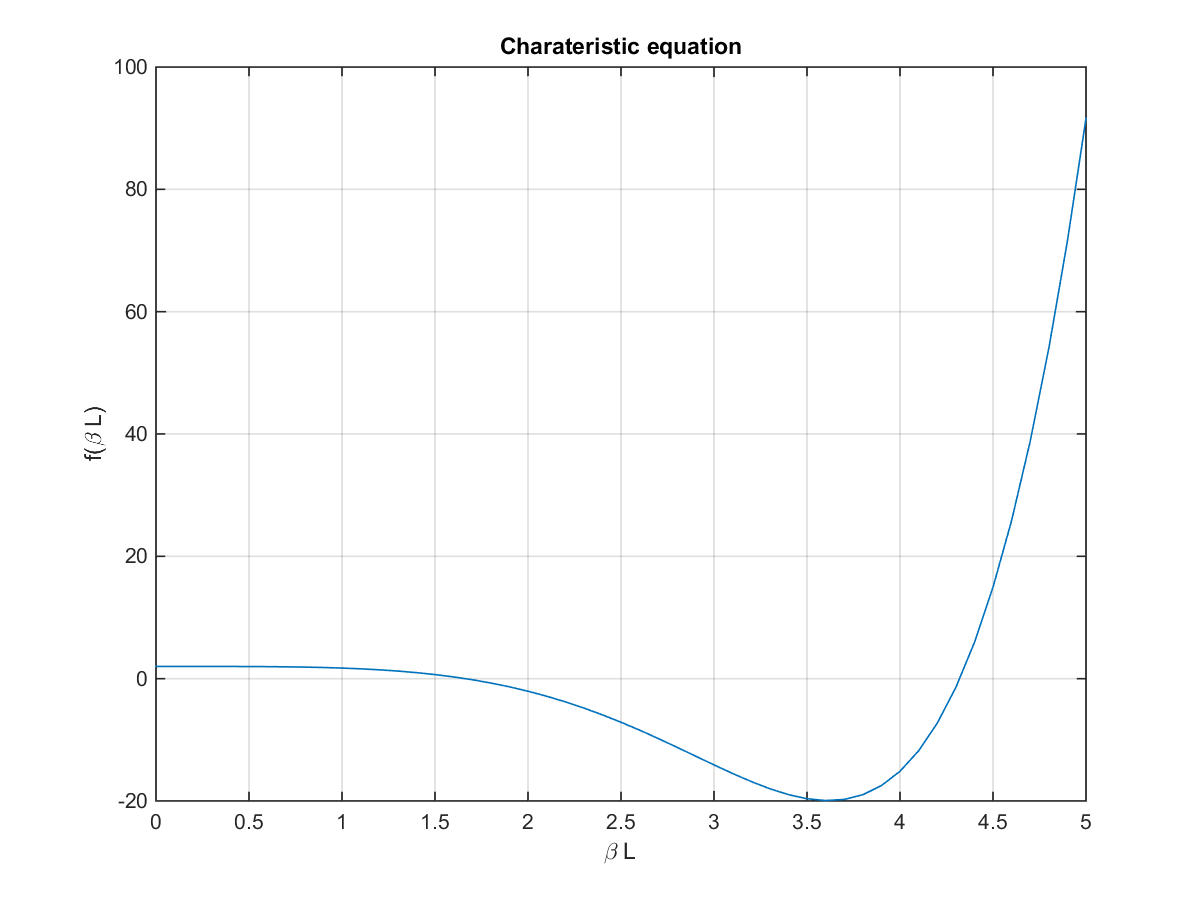
\includegraphics[scale=0.5]{hw2_VB2.png}
		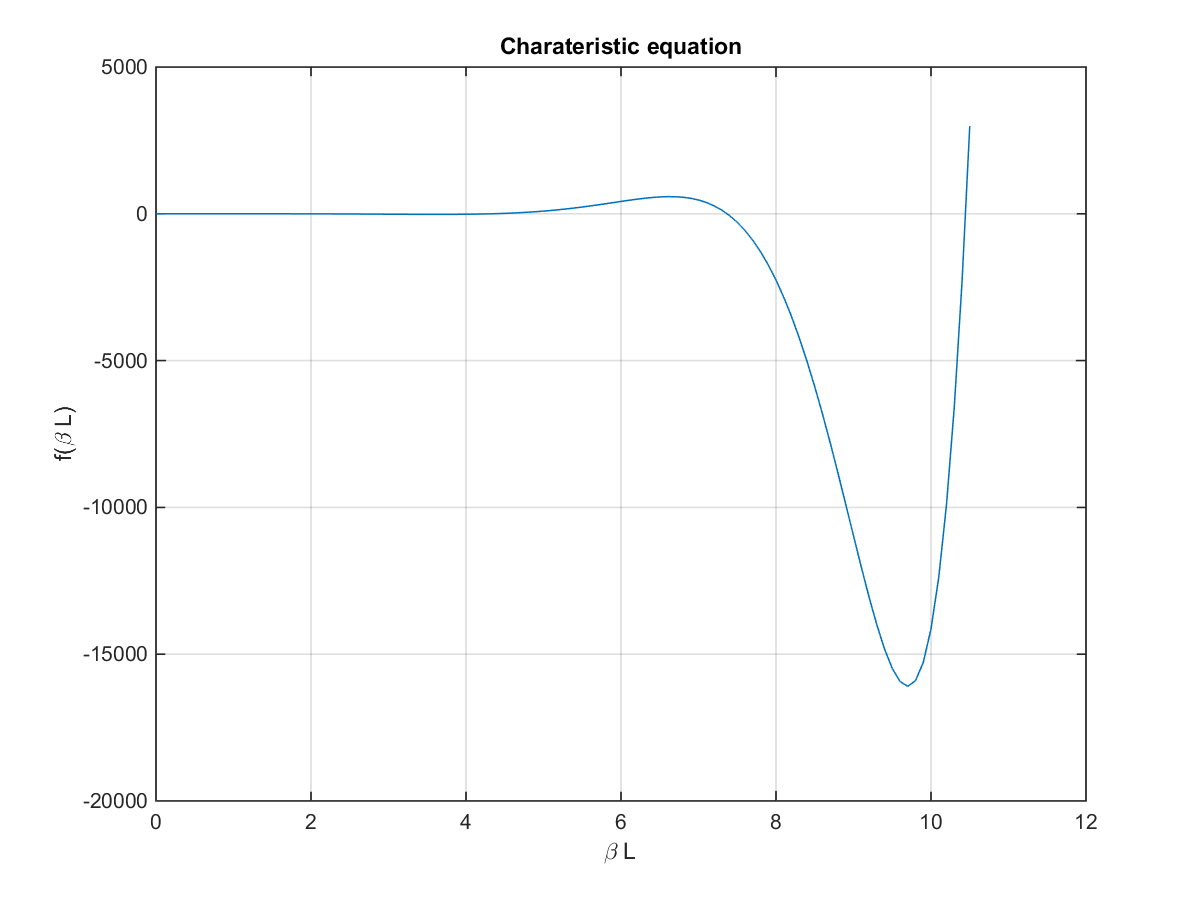
\includegraphics[scale=0.5]{hw2_VB1.png}
	\end{figure}\\
	The first four nonzero roots of characteristic equation are: $\beta_1L = 1.665, \beta_2L = 4.322, \beta_3L = 7.37 $ and $\beta_4L = 10.45$\\
	Natural frequencies is defined from computed values of $\beta$, we have:\\
	since: $ \beta^4 = \dfrac{\rho A\omega^2}{EI} \Rightarrow \omega = \beta^2\sqrt{\dfrac{EI}{\rho A}} = (\beta L)^2\sqrt{\dfrac{EI}{\rho AL^4}}$\\
	we first have: $\sqrt{\dfrac{EI}{\rho AL^4}} = \sqrt{\dfrac{68.9\bullet 10^9 \times 6.69\bullet 10^{-11}}{2.7\bullet10^6 \times 78.4\bullet10^{-6}\times 0.46^4}} \approx 0.7$\\
	$\beta_1L = 1.665 \Rightarrow \omega_1 = (\beta_1L)^2\bullet 0.7 = 1.665^2\bullet 0.7 = 1.94$ rad/s\\
	$\beta_2L = 4.322 \Rightarrow \omega_1 = (\beta_2L)^2\bullet 0.7 = 4.322^2\bullet 0.7 = 13.07$ rad/s\\
	$\beta_3L = 7.37 \Rightarrow \omega_1 = (\beta_3L)^2\bullet 0.7 = 7.37^2\bullet 0.7 = 38.02$ rad/s\\
	$\beta_4L = 10.45 \Rightarrow \omega_1 = (\beta_4L)^2\bullet 0.7 = 10.45^2\bullet 0.7 = 76.4$ rad/s\\
	
	The mode shape can be written as:\\
	$\bar{Y}_i(X) = \left(\dfrac{A}{B}\right)_i\left(\cosh(\beta_iL\dfrac{X}{L}) - \cos(\beta_iL\dfrac{X}L)\right) + \sinh(\beta_iL\dfrac{X}{L}) - \sin(\beta_iL\dfrac{X}{L})$\\
	with: 	$\left(\dfrac{A}{B}\right)_i =  -\dfrac{ \sinh\beta_iL + \sin \beta_iL}{\cosh \beta_iL + \cos \beta_iL} $\\
	we have the table result:
	\begin{tabular} {c c c c c}
		$\beta L$ & 1.575 & 4.226 & 7.282 & 10.371 \\
		$a/b$ & -1.341 & -0.985 & -1.0005 & 1
	\end{tabular}\\
	$\bar{Y}_1(X) = -1.341\left(\cosh(1.665\dfrac{X}{0.46}) - \cos(1.665\dfrac{X}{0.46})\right) + \sinh(1.665\dfrac{X}{0.46}) - \sin(1.6655\dfrac{X}{0.46})$\\	
	\hspace*{0.9cm} $= -1.341\left(\cosh(3.62X) - \cos(3.62X)\right) + \sinh(3.62X) - \sin(3.62X)$\\	
	$\bar{Y}_2(X) = -0.985\left(\cosh(4.322\dfrac{X}{0.46}) - \cos(4.322\dfrac{X}{0.46})\right) + \sinh(4.322\dfrac{X}{0.46}) - \sin(4.322\dfrac{X}{0.46})$\\	
	\hspace*{0.9cm} $= -0.985\left(\cosh(9.4X) - \cos(9.4X)\right) + \sinh(9.4X) - \sin(9.4X)$\\
	$\bar{Y}_3(X) = -1.0005\left(\cosh(7.37\dfrac{X}{0.46}) - \cos(7.37\dfrac{X}{0.46})\right) + \sinh(7.37\dfrac{X}{0.46}) - \sin(7.37\dfrac{X}{0.46})$\\	
	\hspace*{0.9cm} $= -1.0005\left(\cosh(16.02X) - \cos(16.02X)\right) + \sinh(16.02X) - \sin(16.02X)$\\
	$\bar{Y}_4(X) = -1\left(\cosh(10.45\dfrac{X}{0.46}) - \cos(10.45\dfrac{X}{0.46})\right) + \sinh(10.45\dfrac{X}{0.46}) - \sin(10.45\dfrac{X}{0.46})$\\	
	\hspace*{0.9cm} $= -\cosh(22.72X) + \cos(22.71X) + \sinh(22.72X) - \sin(22.72X)$\\
	\begin{figure}[htp]
		\centering
		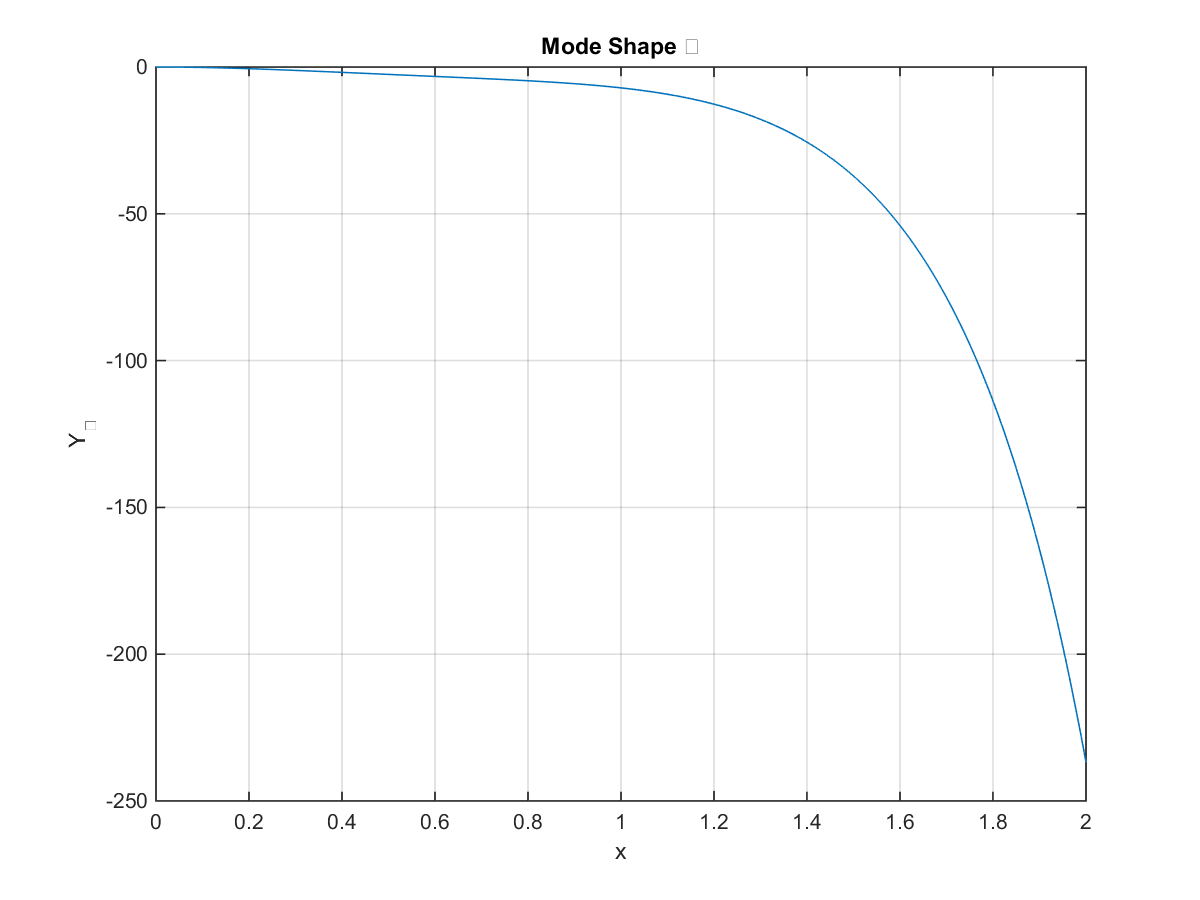
\includegraphics[scale=0.5]{hw2_VB_mode1.png}
		\caption{Mode Shape 1}
	\end{figure}\\
	\begin{figure}[htp]
		\centering
		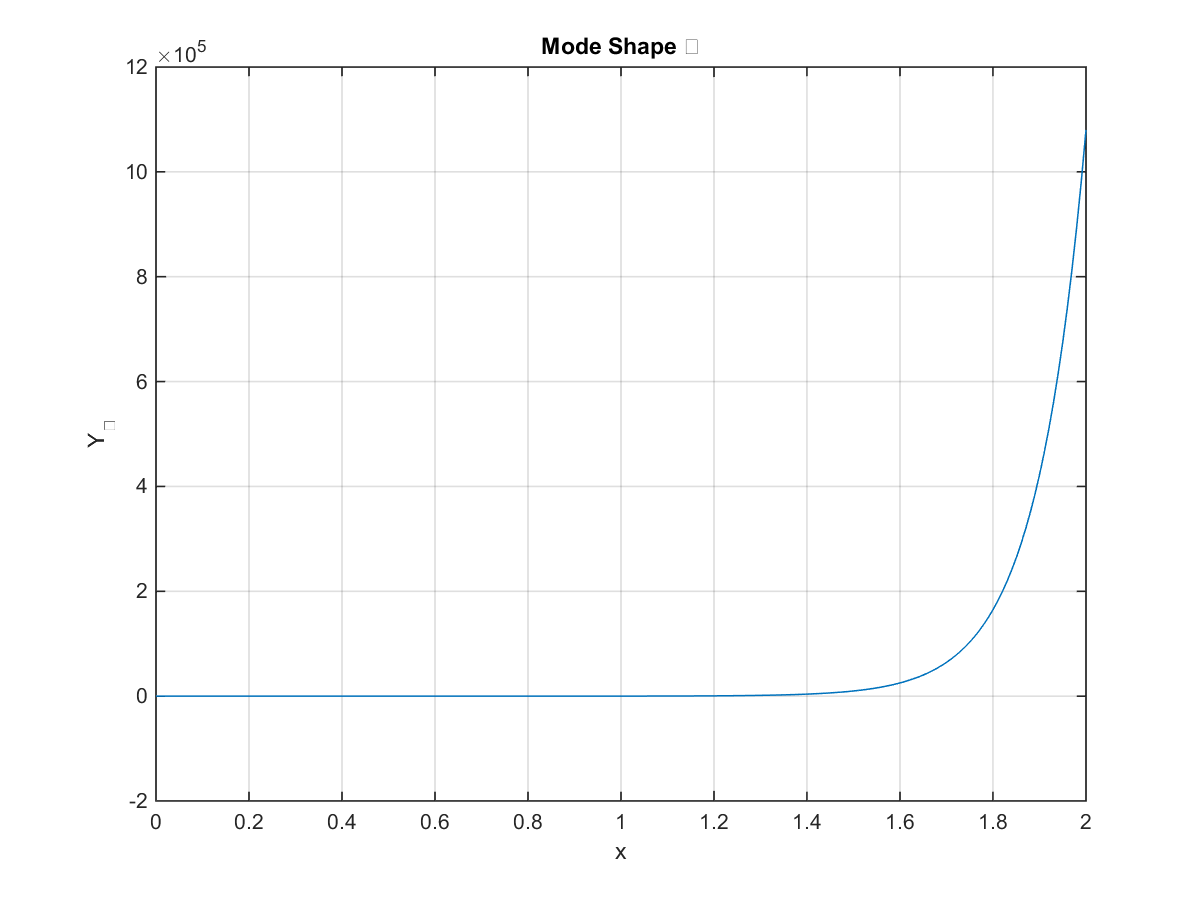
\includegraphics[scale=0.5]{hw2_VB_mode2.png}
		\caption{Mode Shape 2}
		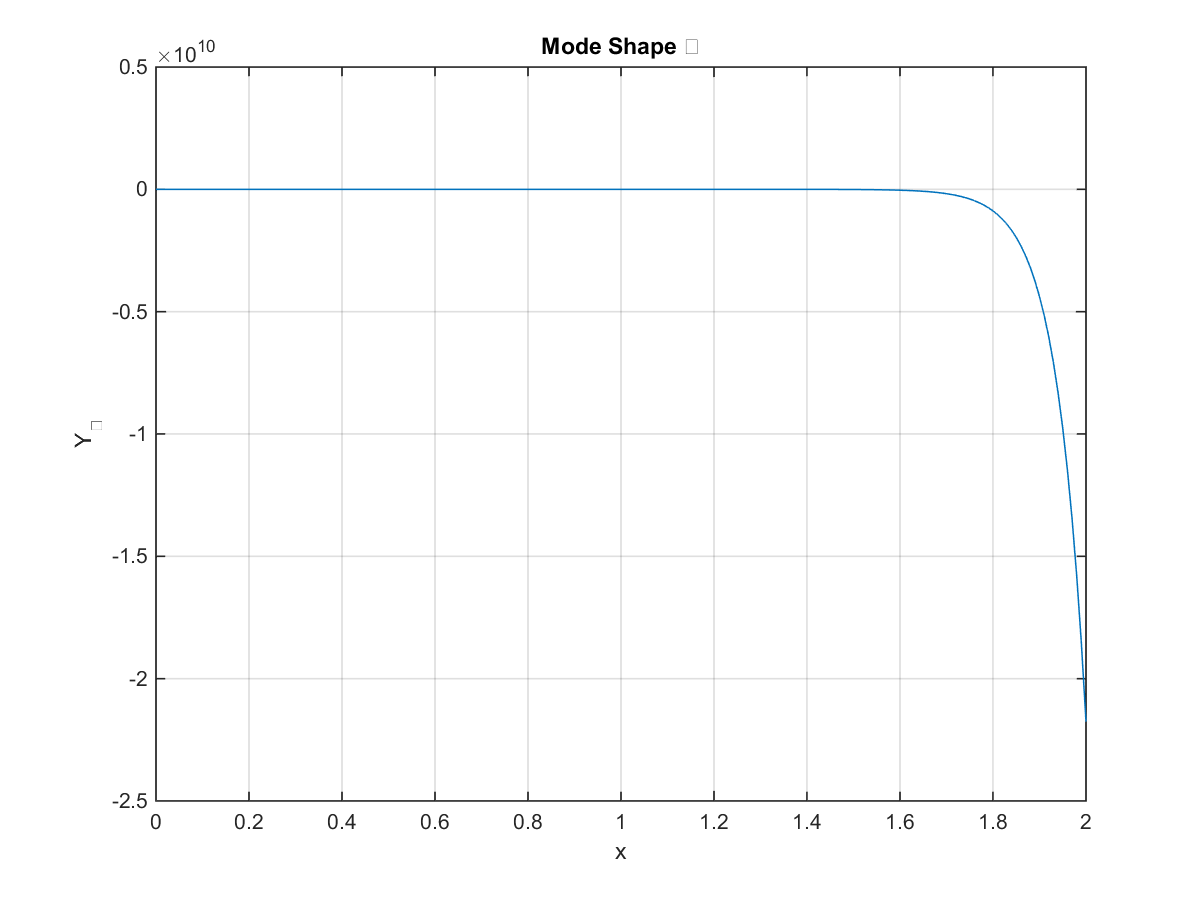
\includegraphics[scale=0.5]{hw2_VB_mode3.png}
		\caption{Mode Shape 3}
		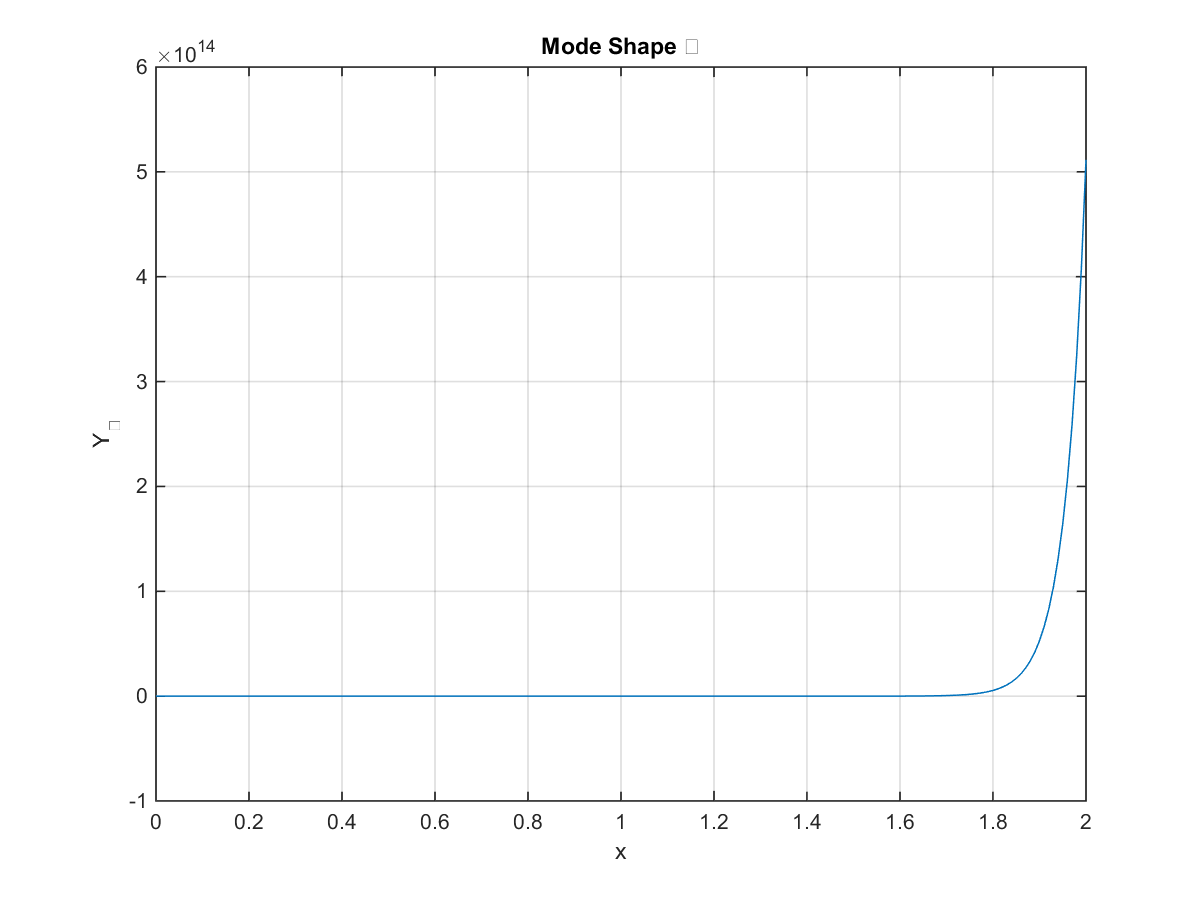
\includegraphics[scale=0.5]{hw2_VB_mode4.png}
		\caption{Mode Shape 4}
	\end{figure}\\
	\pagebreak
	
	
	\item Modeled the tip mass as a solid having mass and inertia:\\
	- The first two bound conditions are same with above: we have equation (3) and (4)\\
	- From the rotational inertial we form the third and forth condition:\\
	\hspace*{2cm} $\dfrac{a}{b} = -\dfrac{k_1(\sinh\beta L - \sin\beta L) + (\cosh\beta L + \cos\beta L)}{k_1(\cosh\beta L + \cos\beta L) + (\sinh\beta L - \sin\beta L)}$	\hspace{2cm} (7)\\	
	\hspace*{2cm} $\dfrac{a}{b} = -\dfrac{k_2(\cosh\beta L - \cos\beta L) - (\sinh\beta L + \sin\beta L)}{k_2(\sinh\beta L + \sin\beta L) - (\cosh\beta L + \cos\beta L)}$ \hspace{2cm} (8)\\
	with $k_1 = \dfrac{\bar{M}}{m}\beta L = 0.1508\beta L$\\
	The rotary inertia is: $I_0 = \dfrac{1}{4}M_1r_1^2 + \dfrac{1}{3}M_1h_1^2 + M_2h_2^2$\\
	\hspace*{3.8cm} $ = \pi*1.15^2\times10^{-4}*1.13\times10^{-2}*2.7\times10^6\left( \dfrac{1}{4}1.15^2\times10^{-4} + \dfrac{1}{3}1.13^2\times10^{-4}\right) \\ \hspace*{4.4cm} + \pi*0.45^2\times10^{-4}*1.17\times10^{-2}*2.7\times10^6*1.17^2\times10^{-4}$\\
	\hspace*{3.8cm} $ = 1.234\times 10^{-3}$ \\
	So the rotary term for $k_2$ is: $k_2 = \dfrac{I_0}{mL^2}(\beta L)^3 = \dfrac{1.234\times10^{-3}}{97.4\times10^{-3}*0.46^2}(\beta L)^3 = 0.06(\beta L)^3 $\\
	Characteristic equation:\\
	$(k_1k_2-1)(\cosh\beta L\cos\beta L) - (k_1k_2 +1) + (k_1 + k_2)(\cosh\beta L\sin\beta L) -(k_1-k_2)(\sinh\beta L\cos\beta L) = 0 \\
	\Leftrightarrow (9.048\times10^{-3}(\beta )^4-1)(\cosh\beta L\cos\beta L) - (9.048\times10^{-3}(\beta )^4+1) + (0.1508\beta L + 0.06(\beta L)^3)(\cosh\beta L\sin\beta L) - (0.1508\beta L - 0.06(\beta L)^3)(\sinh\beta L\cos\beta L) = 0$ 
	\begin{figure}[htp]
		\centering
		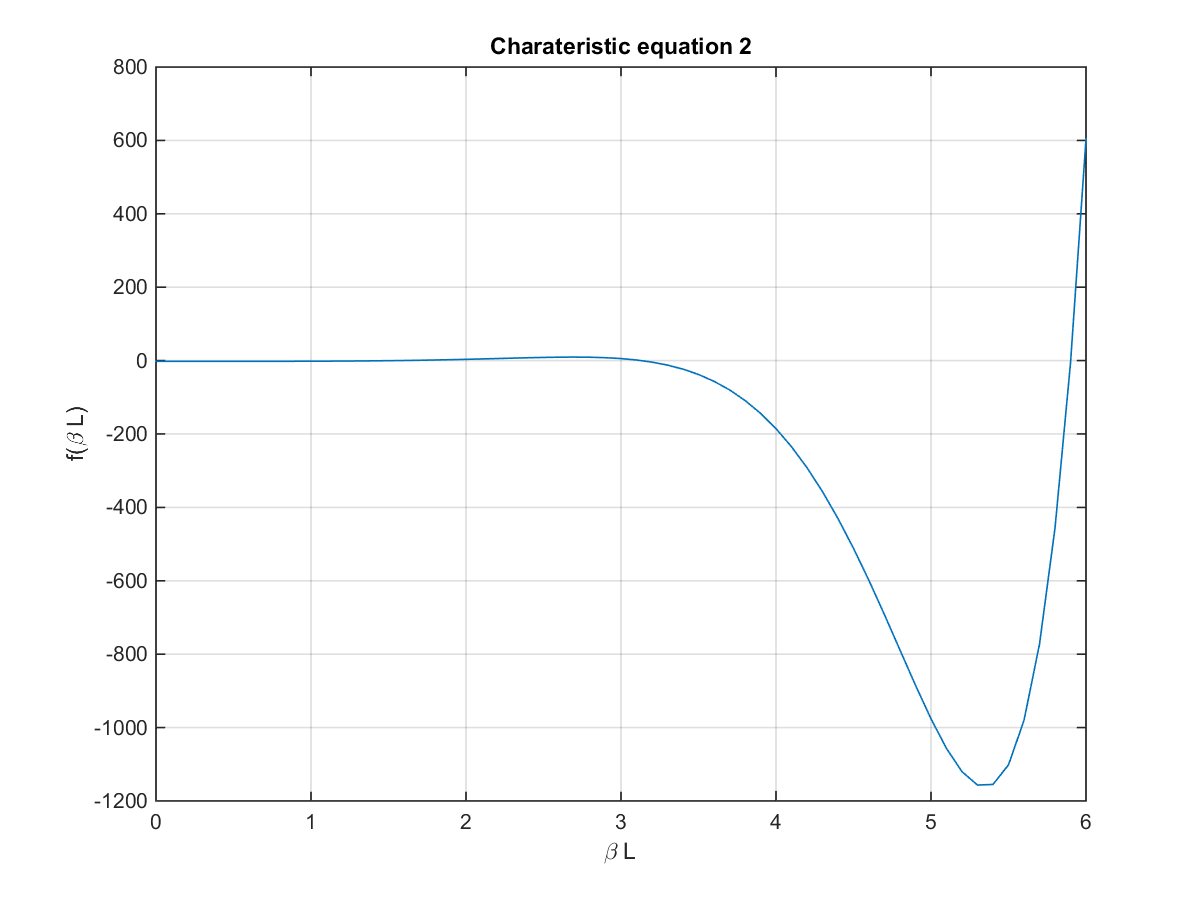
\includegraphics[scale=0.4]{hw2_VB3.png}
		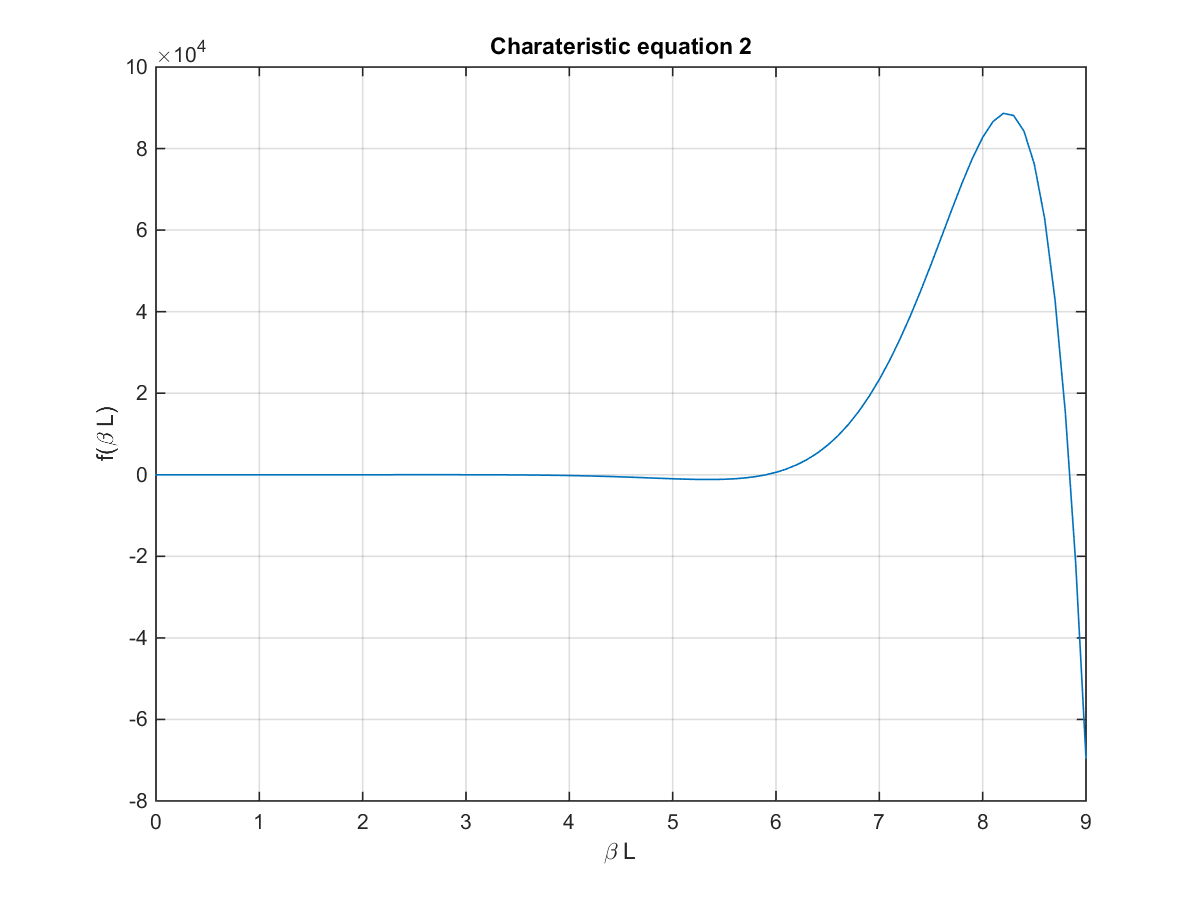
\includegraphics[scale=0.4]{hw2_VB4.png}
	\end{figure}\\
	The first four nonzero roots of characteristic equation are: $\beta_{21}L = 1.55, \beta_{22}L = 3.13, \beta_{23}L = 5.9 $ and $\beta_{24}L = 8.84$\\
	Natural frequencies is defined from computed values of $\beta$, we have: \\
	\hspace*{3cm} $\omega_n^2 = \beta^4\dfrac{EIL}{m} \Leftrightarrow \omega_n = (\beta L)^2\sqrt{\dfrac{EI}{mL^3}}$\\
	with: \hspace{1cm} 	$\sqrt{\dfrac{EI}{mL^3}} = \sqrt{\dfrac{68.9\bullet 10^9 \times 6.69\bullet 10^{-11}}{97.4\bullet10^{-3}\times 0.46^3}} \approx 22.05$\\
	The first four natural frequencies of vibration are defined:
	\begin{center}
	\begin{tabular} {c c c c c}
		$\beta L$ & 1.55 & 3.13 & 5.9 & 8.84 \\
		$\omega_n$ & 53 & 216.3 & 767.9 & 1725
	\end{tabular}
	\end{center}
	The mode shape can be written as:\\
	$\bar{Y}_i(X) = \left(\dfrac{A}{B}\right)_i\left(\cosh(\beta_iL\dfrac{X}{L}) - \cos(\beta_iL\dfrac{X}L)\right) + \sinh(\beta_iL\dfrac{X}{L}) - \sin(\beta_iL\dfrac{X}{L})$\\
	with: 	$\left(\dfrac{a}{b}\right)_i = -\dfrac{k_{1i}(\sinh\beta_iL - \sin\beta_iL) + (\cosh\beta_iL + \cos\beta_iL)}{k_{1i}(\cosh\beta_iL + \cos\beta_iL) + (\sinh\beta_iL - \sin\beta_iL)}$\\
	we have the table result:
	\begin{tabular} {c c c c c}
		$\beta L$ & 1.55 & 3.13 & 5.9 & 8.84 \\
		$a/b$ & -1.52 & -0.97 & -1.0002 & 1
	\end{tabular}\\
	$\bar{Y}_1(X) = -1.52\left(\cosh(1.55\dfrac{X}{0.46}) - \cos(1.55\dfrac{X}{0.46})\right) + \sinh(1.55\dfrac{X}{0.46}) - \sin(1.55\dfrac{X}{0.46})$\\	
	\hspace*{0.9cm} $= -1.52\left(\cosh(3.37X) - \cos(3.37X)\right) + \sinh(3.37X) - \sin(3.37X)$\\	
	$\bar{Y}_2(X) = -0.97\left(\cosh(3.13\dfrac{X}{0.46}) - \cos(3.13\dfrac{X}{0.46})\right) + \sinh(3.13\dfrac{X}{0.46}) - \sin(3.13\dfrac{X}{0.46})$\\	
	\hspace*{0.9cm} $= -0.97\left(\cosh(6.8X) - \cos(6.8X)\right) + \sinh(6.8X) - \sin(6.8X)$\\
	$\bar{Y}_3(X) = -1.0002\left(\cosh(5.9\dfrac{X}{0.46}) - \cos(5.9\dfrac{X}{0.46})\right) + \sinh(5.9\dfrac{X}{0.46}) - \sin(5.9\dfrac{X}{0.46})$\\	
	\hspace*{0.9cm} $= -1.0002\left(\cosh(12.83X) - \cos(12.83X)\right) + \sinh(12.83X) - \sin(12.83X)$\\
	$\bar{Y}_4(X) = -1\left(\cosh(8.84\dfrac{X}{0.46}) - \cos(8.84\dfrac{X}{0.46})\right) + \sinh(8.84\dfrac{X}{0.46}) - \sin(8.84\dfrac{X}{0.46})$\\	
	\hspace*{0.9cm} $= -\cosh(19.22X) + \cos(19.22X) + \sinh(19.22X) - \sin(19.22X)$
	\begin{figure}[htp]
		\centering
		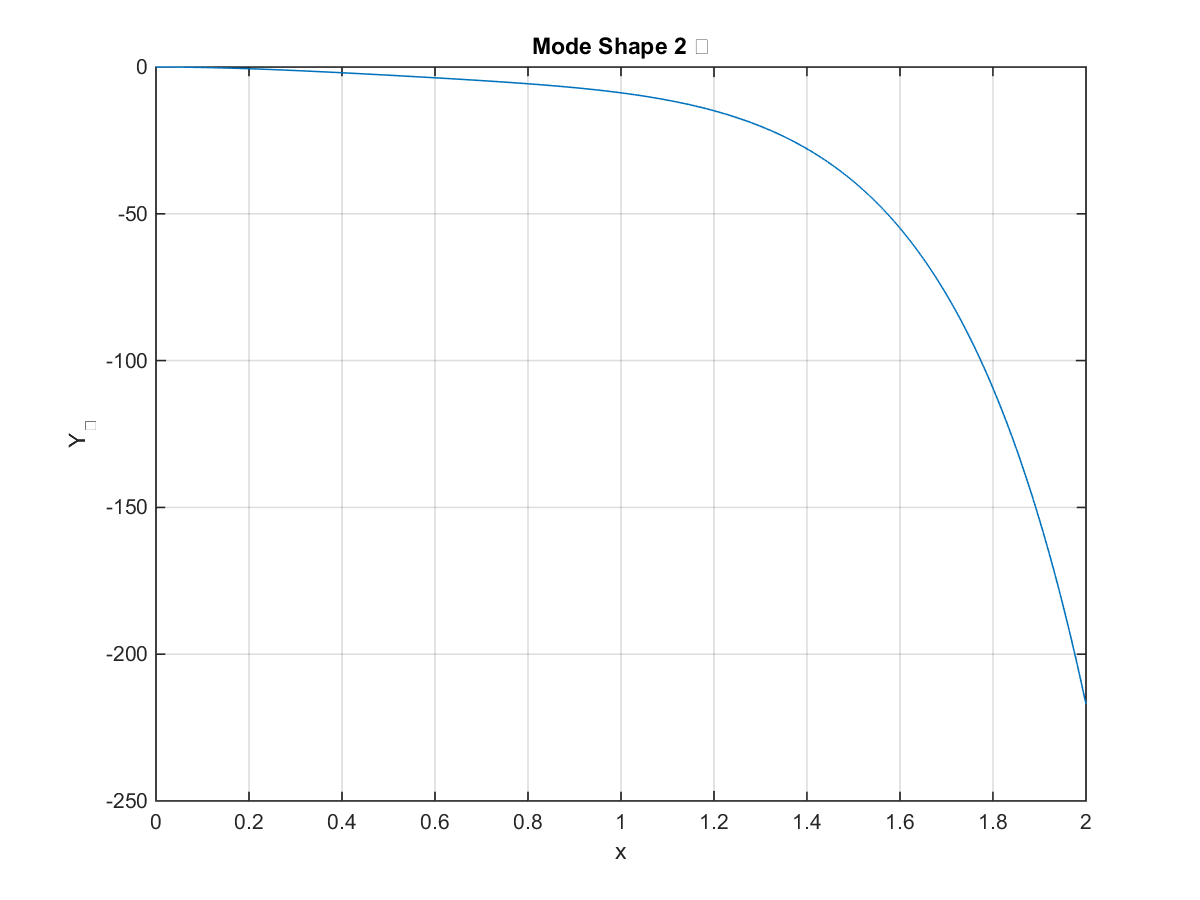
\includegraphics[scale=0.5]{hw2_VB2_mode1.png}
		\caption{Mode Shape 2-1}
	\end{figure}
	\begin{figure}[htp]
		\centering
		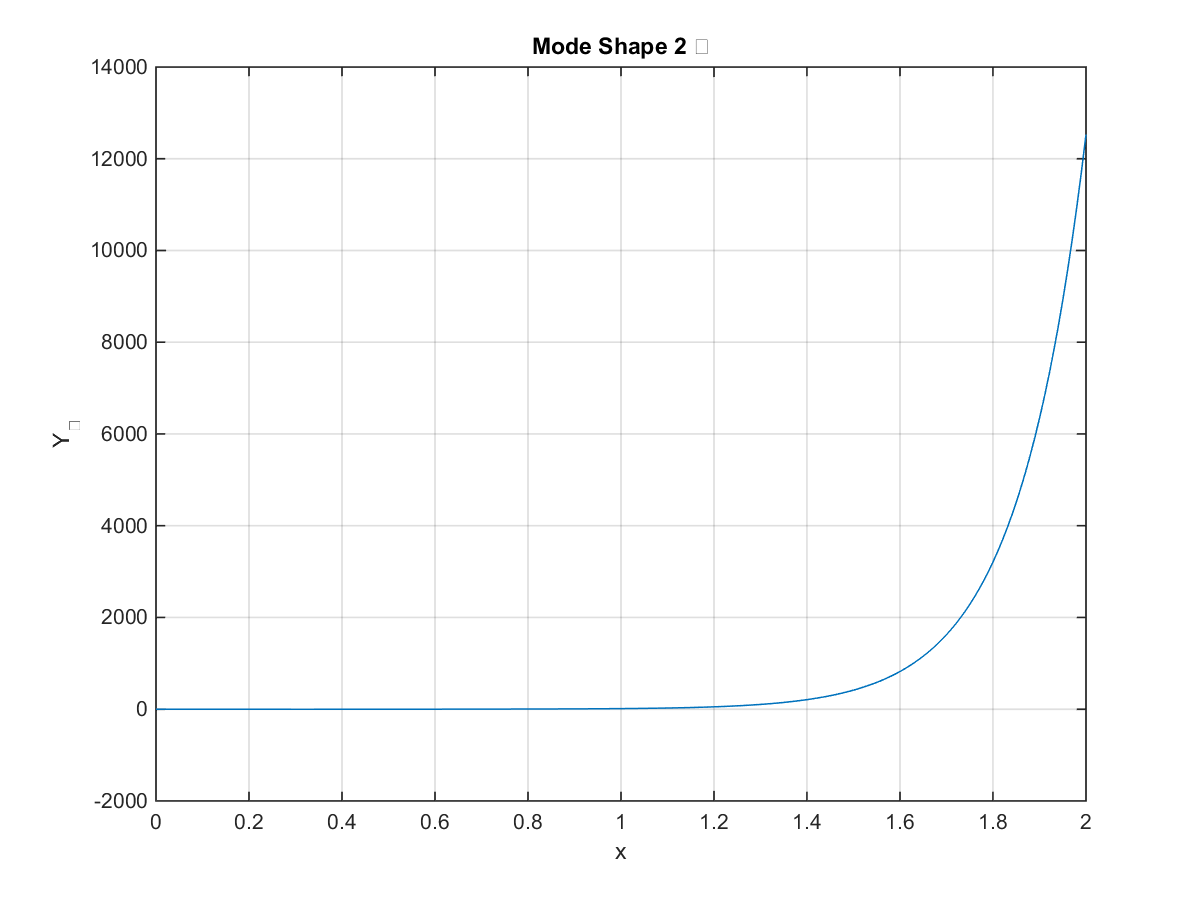
\includegraphics[scale=0.5]{hw2_VB2_mode2.png}
		\caption{Mode Shape 2-2}
		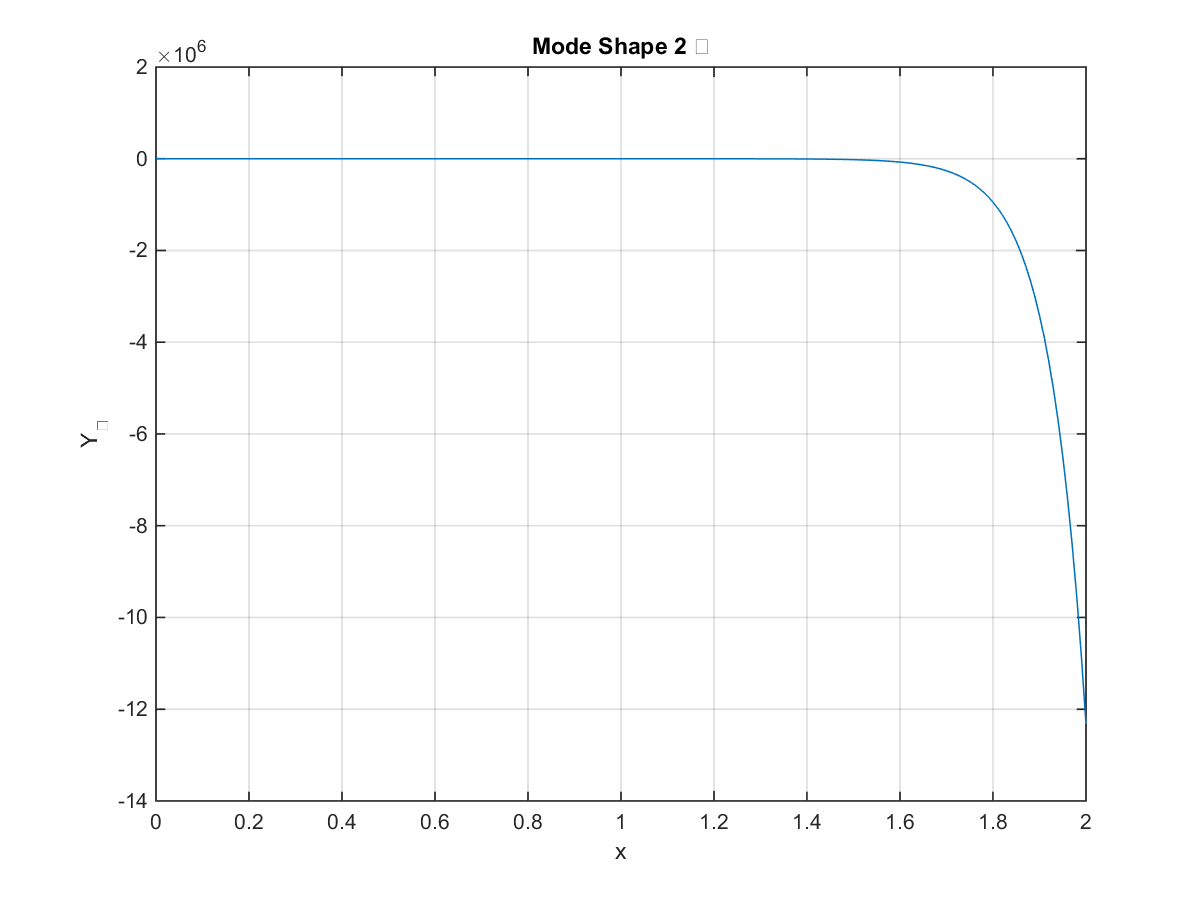
\includegraphics[scale=0.5]{hw2_VB2_mode3.png}
		\caption{Mode Shape 2-3}
		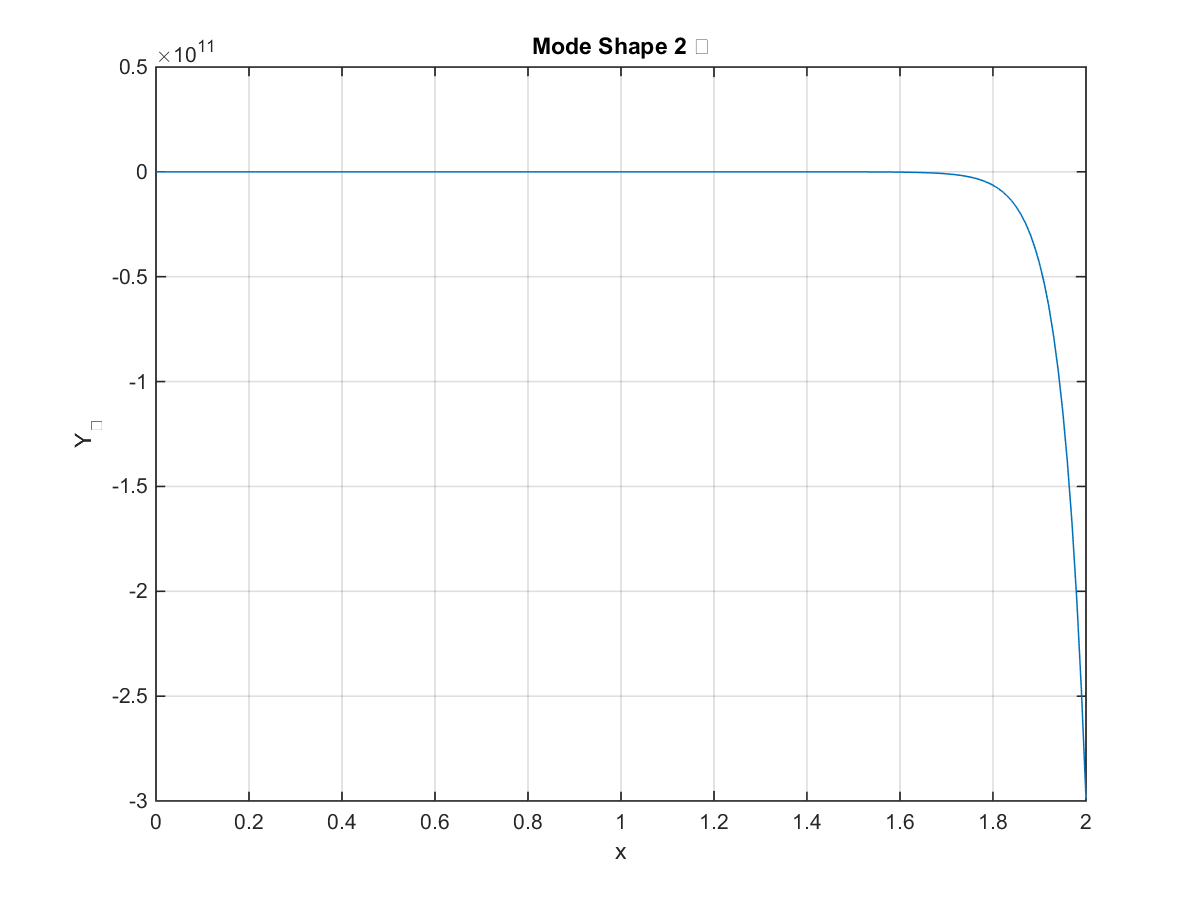
\includegraphics[scale=0.5]{hw2_VB2_mode4.png}
		\caption{Mode Shape 2-4}
	\end{figure}	
	
\end{enumerate}

\end{document}